\documentclass[conference]{IEEEtran}
\usepackage{amsmath,amssymb}
\usepackage{graphicx}
\usepackage{booktabs}
\usepackage{multirow}
\usepackage{url}
\usepackage{cite}
\usepackage{stfloats} % allow double-column (figure*) floats at page bottom too, not just top

\begin{document}

\title{Graph-Based Polypharmacy Risk Networks for Adverse Event Prediction in ICU Patients: A MIMIC-IV Analysis}

\author{
\IEEEauthorblockN{Author Name}
\IEEEauthorblockA{Affiliation \\ Email}
}

\maketitle

\begin{abstract}
Polypharmacy -- the concurrent use of multiple medications -- is common in
intensive care and is a recognized driver of adverse events, yet most
machine-learning studies on MIMIC-IV target mortality prediction rather than
modeling drug-interaction risk directly. We address this gap by constructing
a population-level drug co-administration graph from 9{,}974 adult ICU stays
and comparing three patient-level feature representations -- node2vec graph
embeddings, hand-crafted graph-theoretic statistics, and a one-hot tabular
baseline -- for predicting three polypharmacy-relevant outcomes: acute kidney
injury (AKI, KDIGO-based), a delirium proxy, and a bleeding proxy. Across four
classifiers and stratified 5-fold cross-validation, we find a mixed but
interpretable pattern: the tabular baseline wins when given unrestricted
access to drug identity (AKI AUROC 0.763, bleeding AUROC 0.864), while graph
embeddings outperform a leakage-corrected tabular baseline for delirium
(AUROC 0.876 vs.\ 0.858, paired bootstrap $\Delta$=+0.018, 95\% CI
[0.011, 0.025], $p<0.0001$), replicating on an independent, zero-overlap
second subsample ($\Delta$=+0.015). We further report a label-leakage
correction identified during development (delirium label circularity with
tabular drug features, corrected AUROC $0.944 \rightarrow 0.858$) and
perturbation-based, reliability-filtered drug-risk rankings. This comparison
is evidence for when graph-based representations add value over tabular
baselines in EHR-based polypharmacy modeling.
\end{abstract}

\begin{IEEEkeywords}
polypharmacy, graph embeddings, node2vec, MIMIC-IV, electronic health records, acute kidney injury, delirium, adverse drug events
\end{IEEEkeywords}

\section{Introduction}

Adverse drug events are among the most common preventable harms in
critical care, and polypharmacy -- the concurrent administration of
multiple medications -- is their most consistent upstream driver. Nearly
every patient in the intensive care unit (ICU) receives multiple concurrent
medications, and the resulting combinations are mechanistically linked to
nephrotoxicity, delirium, and bleeding complications. Despite this,
machine-learning research on the MIMIC-IV critical care database has
concentrated overwhelmingly on a narrow set of targets -- in-hospital
mortality, length of stay, and readmission -- leaving polypharmacy-specific
adverse event modeling comparatively
underexplored~\cite{harutyunyan2019benchmarking,rohr2024revisiting}. As a
result, the \emph{combinatorial} structure of drug co-administration --
which drugs are given together, how often, and to whom -- is rarely modeled
explicitly; most prior EHR risk models instead treat medication exposure as
an unordered feature bag, discarding the co-administration structure
entirely.

This paper asks a narrower, more falsifiable question than ``can graphs
model polypharmacy risk'': under what conditions does a graph-based
representation of drug co-administration outperform a conventional tabular
representation built from the same underlying information? Answering this
requires holding everything else fixed -- cohort, labels, classifiers,
cross-validation protocol -- and varying only the feature representation,
which is the design we adopt here. We build a population-level
co-administration graph over generic drug names, learn
node2vec~\cite{grover2016node2vec} embeddings for each drug, and compare
three patient-level feature representations head-to-head -- graph
embedding, graph-theoretic statistics, and a tabular one-hot baseline -- for
three clinically distinct outcomes: acute kidney injury (AKI), a delirium
proxy, and a bleeding proxy.

Our contribution is threefold: (1) a three-way feature-representation
comparison evaluated under matched conditions across three clinically
distinct outcomes, rather than a single-outcome demonstration; (2) a
documented and corrected label-leakage circularity between the delirium
outcome definition and tabular drug features -- a failure mode consistent
with broader findings on leakage-driven overoptimism in health-care machine
learning~\cite{davis2023labelleakage,kapoor2023leakage} -- together with a
paired significance test validating the corrected result; and (3) a
confirmatory replication of the headline result on an independent,
zero-overlap cohort subsample, directly addressing the generalizability
concern that any single-subsample result invites.

\section{Related Work}

\textbf{MIMIC-based clinical prediction.} The MIMIC-IV critical care
database~\cite{johnson2023mimiciv}, and MIMIC-III before it, have enabled a
large body of ICU outcome-prediction research, but that research is heavily
concentrated on a narrow set of targets.
Harutyunyan et al.~\cite{harutyunyan2019benchmarking} formalized this as a
standard benchmark suite of four tasks -- in-hospital mortality,
length-of-stay, decompensation, and phenotyping -- and the great majority of
subsequent MIMIC-based deep learning papers evaluate against some subset of
these same targets. This concentration has persisted into the MIMIC-IV era:
recent work revisiting clinical outcome prediction specifically for MIMIC-IV
continues to organize its tasks around diagnosis, procedure, length-of-stay,
and routing prediction~\cite{rohr2024revisiting}. Polypharmacy-specific
adverse event modeling, by contrast, has received comparatively little
direct attention despite polypharmacy's well-established mechanistic link to
nephrotoxicity, delirium, and bleeding; this concentration on
mortality/LOS-style targets is the specific gap this paper addresses.

\textbf{Graph and network representation learning.} The embedding method we
use, node2vec~\cite{grover2016node2vec}, extends
DeepWalk~\cite{perozzi2014deepwalk} by generalizing random-walk sampling
with biased second-order walks, learning a vector representation for each
node such that nodes appearing in similar random-walk contexts receive
similar embeddings. This family of methods was first brought into the
clinical setting by Med2Vec~\cite{choi2016med2vec}, which learns
medical-code embeddings from the co-occurrence structure of codes within a
clinical visit -- structurally close to how we treat drug co-occurrence
within an admission -- and by GRAM~\cite{choi2017gram}, which supplements
code embeddings with a medical ontology graph via attention to address data
sparsity. More recent work has extended graph-based EHR representation to
heterogeneous, multi-task settings: MulT-EHR mines relations across a
heterogeneous graph for simultaneous multi-task prediction -- drug
recommendation, length-of-stay, mortality, and readmission -- on MIMIC-III
and MIMIC-IV~\cite{chan2024multehr}. All of this work targets
diagnosis/procedure codes or general EHR heterogeneity broadly, rather than
drug co-administration specifically, and none runs a matched
embedding-vs-tabular-baseline comparison of the kind we report here.

\textbf{Polypharmacy and drug-interaction graph modeling.} The most directly
related prior work is Decagon~\cite{zitnik2018decagon}, which models
polypharmacy side effects with a graph convolutional network over a
multimodal graph of protein-protein interactions, drug-protein targets, and
drug-drug interaction edges labeled by side-effect type. Decagon operates at
the molecular/pharmacological level -- predicting which side effect a drug
\emph{pair} may cause from biological interaction data -- whereas our graph
is built directly from \emph{observed} patient-level co-administration in
ICU stays and predicts \emph{patient}-level clinical outcomes (AKI,
delirium, bleeding) rather than drug-pair side-effect labels. A recent
survey of machine-learning approaches to drug-drug interaction prediction
documents the rapid growth of graph neural network methods in this space
alongside persistent challenges around model interpretability,
generalizability, and integration with clinical
workflows~\cite{lu2026ddisurvey} -- but this literature is overwhelmingly
oriented toward predicting drug-pair interaction \emph{labels} from
molecular or knowledge-graph structure, not toward predicting patient
outcomes from observed co-administration. The two framings are
complementary: Decagon's molecular graph could in principle be used to
validate or explain associations our co-administration graph surfaces
empirically, which we note as a concrete direction for future work rather
than attempt here.

\textbf{Outcome-specific prior work.} Prior machine-learning work on our
three outcomes is extensive but methodologically disconnected from the
graph-representation question we ask. A systematic review of AKI prediction
on MIMIC found performance varying widely (AUROC 0.49--0.99) with a high
risk of bias in most models~\cite{vagliano2022akireview}; ICU delirium has
been predicted with screening tools using structured variables and
CAM-ICU-based labels similar to our proxy~\cite{bhattacharyya2022delirium};
and freedom from red-blood-cell transfusion has been used as a bleeding
proxy for ICU patients in MIMIC~\cite{levi2021gibleeding}, structurally the
labeling strategy we adopt. None of this work, however, evaluates
graph-based drug representations against tabular baselines under a matched
protocol -- the comparison this paper contributes.

\textbf{Data leakage in clinical machine learning.} The circularity we
identify and correct for the delirium outcome is an instance of a broader,
well-documented failure mode. Davis et al.~\cite{davis2023labelleakage}
frame when model features constitute label leakage in clinical prediction,
arguing that leakage risk depends on the cadence, perspective, and
applicability of a prediction -- directly relevant to our case, in which
the delirium label is partly defined by drugs that also appear as tabular
features. More broadly, a survey of leakage-driven reproducibility failures
across seventeen fields found leakage inflating results in 294 papers,
sometimes enough to overturn a central claim~\cite{kapoor2023leakage}. We
report our correction with a before/after comparison and a paired
significance test in that same spirit of transparent auditing.

\textbf{Interpretability.} We use SHAP~\cite{lundberg2017shap} for the
tabular baseline's tree-based models, and a perturbation (leave-one-drug-out)
analysis for the graph-embedding models, since raw embedding dimensions are
not individually interpretable in the way SHAP requires.

\section{Methods}
\label{sec:methods}

\subsection{Cohort construction}

We extracted adult patients (age $\geq$18) with a first ICU stay of
length $\geq$24 hours from MIMIC-IV via Google BigQuery, yielding 68{,}013
eligible admissions. For BigQuery cost and local compute tractability, we
drew a fixed-seed random subsample of 10{,}000 admissions (seed=42,
$\approx$14.7\% of the eligible cohort), then excluded admissions with fewer
than 3 distinct administered drugs (no meaningful polypharmacy signal),
yielding a final analytic cohort of $n=9{,}974$. Table~\ref{tab:attrition}
reports the full filtering flow.

\begin{table}[t]
\centering
\caption{Cohort attrition.}
\label{tab:attrition}
\begin{tabular}{lr}
\toprule
Filtering step & $n$ (admissions) \\
\midrule
Adult patients, first ICU stay per admission & 85,242 \\
ICU LOS >= 24h & 68,013 \\
Random subsample (seed=42, compute/cost constraint) & 10,000 \\
>= 3 distinct generic drugs administered & 9,974 \\
Final cohort (all labels attached) & 9,974 \\
\bottomrule
\end{tabular}
\end{table}


This subsampling is a stated scope limitation, not a hidden one: to test
whether headline findings generalize beyond the specific subsample drawn, we
separately replicate our primary result on an independent, zero-overlap
second 10{,}000-admission subsample (Section~\ref{sec:replication}).

\subsection{Outcome labels}

We define three binary outcomes, each an explicit, documented proxy rather
than an adjudicated clinical diagnosis:

\begin{itemize}
\item \textbf{AKI}: KDIGO stage $\geq$1~\cite{khwaja2012kdigo}, computed via
  MIMIC-IV's derived \texttt{kdigo\_stages} table. Positive in 7{,}312/9{,}974
  (73.3\%) of the cohort.
\item \textbf{Delirium (proxy)}: administration of an antipsychotic or
  benzodiazepine commonly used for agitation (haloperidol, quetiapine,
  olanzapine, risperidone, ziprasidone, lorazepam, midazolam, diazepam)
  \textbf{AND} a positive CAM-ICU~\cite{ely2001camicu} chartevent (2 of the
  4 CAM-ICU criteria are directly captured in MIMIC-IV chartevents: altered
  mental status and inattention; the full 4-criterion clinical algorithm is
  not reconstructed). Positive in 2{,}679/9{,}974 (26.9\%).
\item \textbf{Bleeding (proxy)}: a new packed red blood cell (PRBC)
  transfusion order after ICU day 2. Positive in 876/9{,}974 (8.8\%).
\end{itemize}

All three are stated limitations in Section~\ref{sec:limitations}: they are
defensible, literature-grounded proxies, not gold-standard adjudicated
outcomes.

\subsection{Drug co-administration graph}

Prescription records were normalized to approximate generic names via a
documented, deterministic cleaning pipeline (dose/form-suffix stripping plus
a small brand-to-generic synonym dictionary). For each admission, two drugs
are considered co-administered if given on an overlapping calendar day. The
\emph{population-level} co-administration graph aggregates this across the
full cohort: nodes are distinct generic drug names, and edge weight is the
number of distinct admissions in which the pair was co-administered.
Table~\ref{tab:graph_stats} reports summary statistics; Figure~\ref{fig:pop_network}
visualizes the top-60 highest-degree drugs, and Figure~\ref{fig:degree_dist}
shows the full degree distribution.

\begin{table}[t]
\centering
\caption{Population co-administration graph summary statistics.}
\label{tab:graph_stats}
\begin{tabular}{lr}
\toprule
Statistic & Value \\
\midrule
Nodes (distinct drugs) & 2,091 \\
Edges (co-administered pairs) & 160,276 \\
Density & 0.0733 \\
Avg.\ clustering coefficient & 0.0011 \\
Connected components & 5 \\
Mean degree & 153.3 \\
Median degree & 49.0 \\
Max degree & 1573 \\
\bottomrule
\end{tabular}
\end{table}


\begin{figure}[t]
\centering
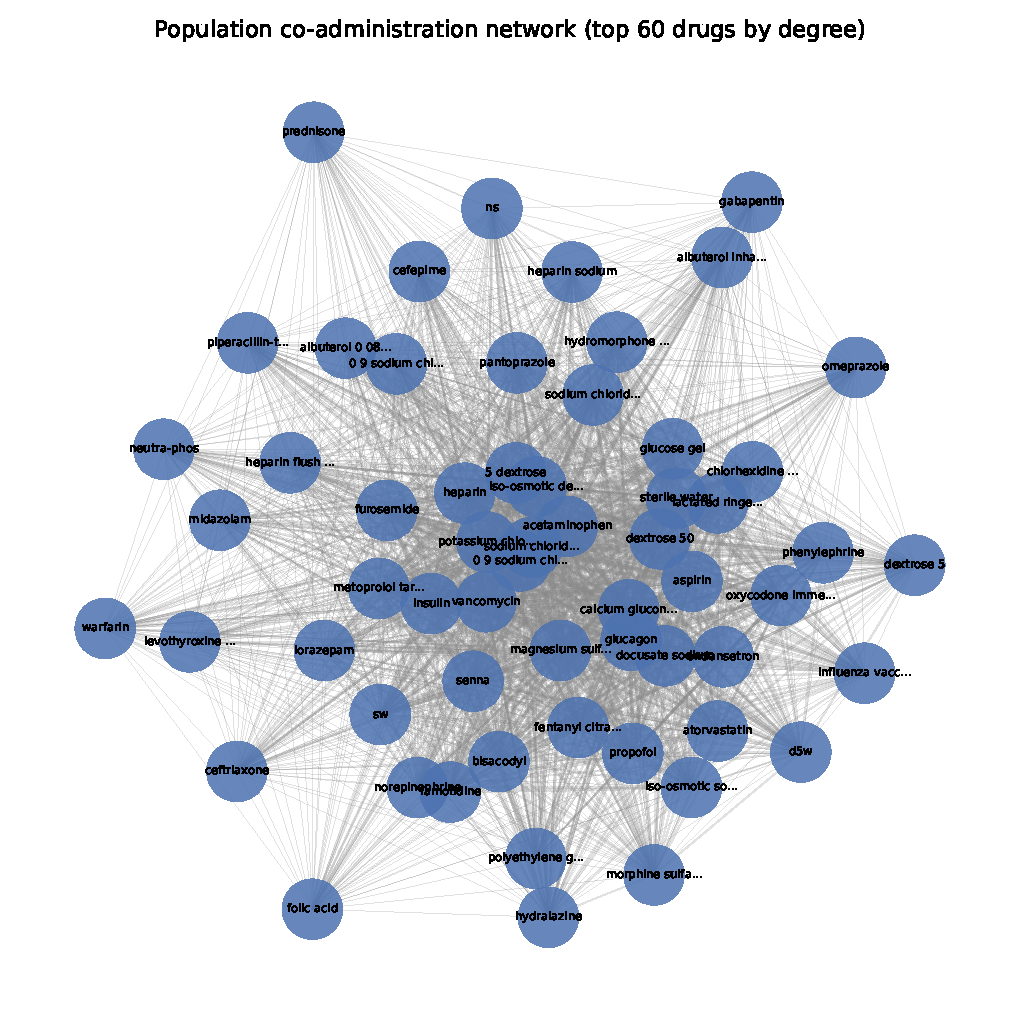
\includegraphics[width=\linewidth]{figures/population_network.pdf}
\caption{Population co-administration network, top 60 drugs by degree. Node size scales with degree; edge width scales with co-administration weight.}
\label{fig:pop_network}
\end{figure}

\begin{figure}[t]
\centering
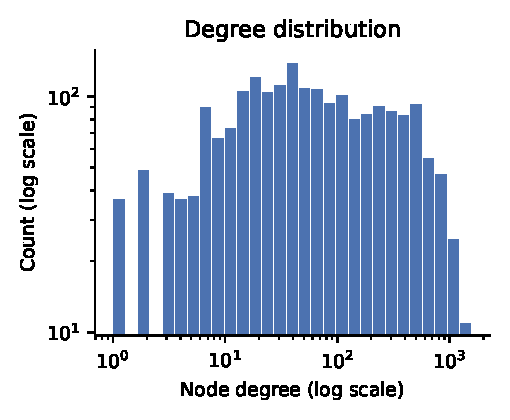
\includegraphics[width=0.85\linewidth]{figures/degree_distribution.pdf}
\caption{Degree distribution of the population co-administration graph (log-log).}
\label{fig:degree_dist}
\end{figure}

\subsection{Feature representations}

We compare three patient-level feature representations, computed for every
admission:

\begin{enumerate}
\item \textbf{Graph embedding}: node2vec~\cite{grover2016node2vec} is trained
  on the weighted population graph (walk length 40, 20 walks per node,
  embedding dimension 64, window 10, default $p{=}1,q{=}1$ -- not
  hyperparameter-tuned, a deliberate choice for a fair, fixed-hyperparameter
  comparison across all three feature sets, discussed further in
  Section~\ref{sec:discussion}). Each patient's feature vector is the mean
  embedding of their administered drugs.
\item \textbf{Graph-theoretic}: sum and max pairwise edge weight among a
  patient's drugs, and the density of their drug-induced subgraph.
\item \textbf{Tabular baseline}: one-hot indicators for every administered
  drug, plus age, sex, and a comorbidity count (distinct ICD diagnosis
  codes).
\end{enumerate}

\subsection{Modeling and evaluation}

For every outcome $\times$ feature-set combination, we train four
classifiers with fixed (untuned) hyperparameters -- logistic regression,
random forest (300 trees), XGBoost~\cite{chen2016xgboost} (300 trees, depth
4), and a 2-layer MLP (64, 32 units) -- under stratified 5-fold
cross-validation, implemented with
scikit-learn~\cite{pedregosa2011scikitlearn}. We report AUROC, AUPRC, F1,
and Brier score, with AUROC 95\% confidence intervals from 1{,}000 bootstrap
resamples of the pooled out-of-fold predictions.

\subsection{Label-leakage correction}

The delirium label is partly \emph{defined} by administration of specific
drugs (Section~III-B); the tabular baseline's one-hot features include
columns for those same drugs, so a tabular model can trivially reconstruct
much of the label via this circularity rather than genuine predictive
signal. We identified this after observing an implausibly high tabular
AUROC (0.944, XGBoost) for delirium. We excluded the delirium-defining drug
columns from the tabular feature set \emph{for the delirium outcome only}
(AKI and bleeding labels are not drug-defined and are unaffected) and refit
all four tabular models, yielding a corrected AUROC of 0.858 (XGBoost).

\section{Results}

\subsection{Three-way feature comparison}

Table~\ref{tab:model_results} reports the full outcome $\times$ feature-set
$\times$ model grid; Figure~\ref{fig:auroc_comparison} summarizes the
best-model AUROC per feature set and outcome. The comparison is mixed rather
than a uniform win for any single representation: the tabular baseline
achieves the highest AUROC for AKI (0.763, XGBoost) and bleeding (0.864,
XGBoost), while the graph embedding achieves the highest AUROC for delirium
(0.876, XGBoost) -- exceeding even the leakage-corrected tabular result
(0.858).

\begin{figure}[t]
\centering
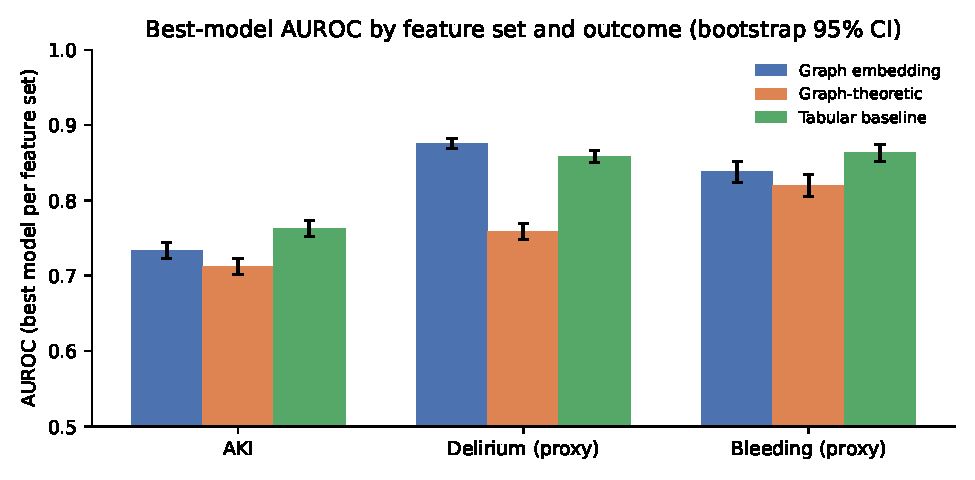
\includegraphics[width=\linewidth]{figures/auroc_comparison.pdf}
\caption{Best-model AUROC by feature set and outcome, with bootstrap 95\% CI error bars.}
\label{fig:auroc_comparison}
\end{figure}

\begin{table*}[t]
\centering
\caption{AUROC (95\% bootstrap CI), AUPRC, F1, and Brier score for every outcome $\times$ feature-set $\times$ model combination. delirium\_label / tabular rows are the leakage-corrected refit (see Section~\ref{sec:methods}).}
\label{tab:model_results}
\begin{tabular}{llllllll}
\toprule
Outcome & Feature set & Model & AUROC & 95\% CI & AUPRC & F1 & Brier \\
\midrule
AKI & Graph embedding & random forest & 0.733 & [0.723, 0.744] & 0.880 & 0.851 & 0.170 \\
 &  & xgboost & 0.726 & [0.716, 0.738] & 0.878 & 0.845 & 0.172 \\
 &  & logistic regression & 0.720 & [0.709, 0.732] & 0.869 & 0.846 & 0.172 \\
 &  & mlp & 0.631 & [0.618, 0.643] & 0.806 & 0.778 & 0.296 \\
AKI & Graph-theoretic & mlp & 0.712 & [0.701, 0.722] & 0.866 & 0.842 & 0.175 \\
 &  & logistic regression & 0.709 & [0.698, 0.720] & 0.863 & 0.843 & 0.176 \\
 &  & xgboost & 0.706 & [0.695, 0.716] & 0.864 & 0.837 & 0.177 \\
 &  & random forest & 0.662 & [0.650, 0.673] & 0.841 & 0.817 & 0.193 \\
AKI & Tabular baseline & xgboost & 0.763 & [0.753, 0.773] & 0.896 & 0.851 & 0.162 \\
 &  & random forest & 0.759 & [0.748, 0.770] & 0.890 & 0.853 & 0.164 \\
 &  & logistic regression & 0.686 & [0.674, 0.697] & 0.848 & 0.808 & 0.210 \\
 &  & mlp & 0.659 & [0.647, 0.670] & 0.841 & 0.779 & 0.294 \\
\addlinespace
Delirium (proxy) & Graph embedding & xgboost & 0.876 & [0.869, 0.883] & 0.735 & 0.625 & 0.121 \\
 &  & random forest & 0.849 & [0.841, 0.858] & 0.710 & 0.569 & 0.133 \\
 &  & mlp & 0.849 & [0.842, 0.857] & 0.664 & 0.621 & 0.182 \\
 &  & logistic regression & 0.849 & [0.841, 0.856] & 0.659 & 0.587 & 0.135 \\
Delirium (proxy) & Graph-theoretic & mlp & 0.759 & [0.748, 0.769] & 0.561 & 0.433 & 0.161 \\
 &  & xgboost & 0.755 & [0.744, 0.765] & 0.551 & 0.419 & 0.162 \\
 &  & logistic regression & 0.738 & [0.727, 0.749] & 0.521 & 0.349 & 0.167 \\
 &  & random forest & 0.718 & [0.707, 0.729] & 0.505 & 0.438 & 0.176 \\
Delirium (proxy) & Tabular baseline & xgboost & 0.858 & [0.850, 0.866] & 0.704 & 0.606 & 0.128 \\
 &  & random forest & 0.848 & [0.839, 0.856] & 0.693 & 0.540 & 0.135 \\
 &  & logistic regression & 0.784 & [0.773, 0.795] & 0.557 & 0.565 & 0.173 \\
 &  & mlp & 0.772 & [0.762, 0.782] & 0.566 & 0.545 & 0.208 \\
\addlinespace
Bleeding (proxy) & Graph embedding & xgboost & 0.838 & [0.824, 0.852] & 0.384 & 0.237 & 0.065 \\
 &  & logistic regression & 0.810 & [0.795, 0.825] & 0.317 & 0.154 & 0.069 \\
 &  & random forest & 0.787 & [0.770, 0.803] & 0.337 & 0.143 & 0.069 \\
 &  & mlp & 0.783 & [0.768, 0.798] & 0.260 & 0.312 & 0.101 \\
Bleeding (proxy) & Graph-theoretic & mlp & 0.821 & [0.806, 0.834] & 0.320 & 0.109 & 0.069 \\
 &  & logistic regression & 0.817 & [0.802, 0.831] & 0.318 & 0.153 & 0.070 \\
 &  & xgboost & 0.807 & [0.792, 0.821] & 0.298 & 0.138 & 0.070 \\
 &  & random forest & 0.761 & [0.743, 0.776] & 0.250 & 0.195 & 0.077 \\
Bleeding (proxy) & Tabular baseline & xgboost & 0.864 & [0.852, 0.875] & 0.442 & 0.338 & 0.062 \\
 &  & random forest & 0.858 & [0.846, 0.870] & 0.431 & 0.157 & 0.064 \\
 &  & mlp & 0.764 & [0.746, 0.779] & 0.267 & 0.326 & 0.122 \\
 &  & logistic regression & 0.722 & [0.703, 0.742] & 0.249 & 0.317 & 0.114 \\
\addlinespace
\bottomrule
\end{tabular}
\end{table*}


We caution that AUPRC for AKI (base rate 73.3\%) should be interpreted
relative to that high base rate rather than in isolation; AUROC is the more
informative metric for this outcome, and we lead with it throughout.

\subsection{Statistical significance of the delirium result}
\label{sec:significance}

Because the embedding-vs-tabular delirium comparison is our headline claim,
we tested it with a paired bootstrap on \emph{identical} cross-validation
fold assignments for both feature sets (rather than comparing two
independently-computed confidence intervals), so the significance estimate
reflects a true paired comparison. Table~\ref{tab:significance} reports the
result: the embedding's AUROC advantage over the leak-free tabular baseline
is statistically significant ($\Delta$=+0.0178, 95\% CI [0.0112, 0.0249],
$p<0.0001$).

\begin{table}[t]
\centering
\caption{Paired bootstrap significance test: node2vec embedding vs.\ leakage-corrected tabular baseline, delirium outcome, identical 5-fold CV splits, 2{,}000 resamples.}
\label{tab:significance}
\begin{tabular}{lr}
\toprule
Quantity & Value \\
\midrule
AUROC (embedding) & 0.8760 \\
AUROC (tabular, leak-free) & 0.8582 \\
Observed $\Delta$AUROC & 0.0178 \\
95\% CI on $\Delta$ & [0.0112, 0.0249] \\
$p$ (approx., two-sided) & 0.0000 \\
\bottomrule
\end{tabular}
\end{table}


\subsection{Confirmatory replication}
\label{sec:replication}

To address whether this result is specific to the particular 10{,}000-admission
subsample drawn, we repeated the entire pipeline -- cohort draw, graph
construction, node2vec training, and the paired significance test -- on a
second, independent subsample with \emph{zero admission overlap} with the
original sample (seed=123, $n=9{,}976$ after filtering). The effect
direction and approximate magnitude replicated
(Table~\ref{tab:replication}): $\Delta$=+0.0152, 95\% CI
[0.0081, 0.0218], overlapping the original sample's confidence interval.

\begin{table}[t]
\centering
\caption{Confirmatory replication on an independent, zero-overlap second 10{,}000-admission subsample (graph and embeddings rebuilt from scratch).}
\label{tab:replication}
\begin{tabular}{lrr}
\toprule
Quantity & Original sample & Replication \\
\midrule
$\Delta$AUROC (emb.\ $-$ tab.) & 0.0178 & 0.0152 \\
95\% CI & [0.0112, 0.0249] & [0.0081, 0.0218] \\
\bottomrule
\end{tabular}
\end{table}


\subsection{Interpretability}

For each outcome's best embedding model, we identify risk-associated drugs
via perturbation analysis: for high-risk patients (top decile of predicted
probability), we remove each drug from their exposure set, re-score, and
average the resulting prediction delta across patients. To avoid reporting
single-patient noise as signal, we exclude any drug supported by fewer than
10 high-risk patients before ranking (Figure~\ref{fig:top_risk_drugs}).
These rankings have \emph{not} been cross-referenced against a clinical
drug-drug-interaction database and should not be interpreted as validated
interactions without that manual check.

\begin{figure*}[!b]
\centering
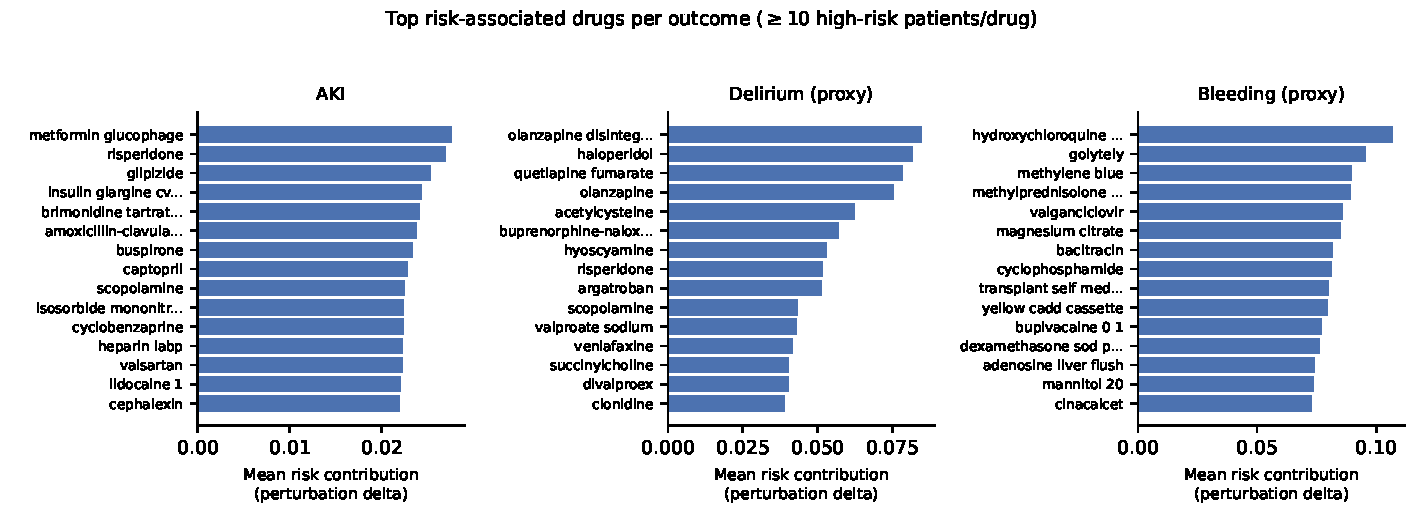
\includegraphics[width=\linewidth]{figures/top_risk_drugs.pdf}
\caption{Top perturbation-ranked risk-associated drugs per outcome (reliability-filtered, $\geq$10 high-risk patients per drug).}
\label{fig:top_risk_drugs}
\end{figure*}

\section{Discussion}
\label{sec:discussion}

The three-way comparison does not support a blanket claim that graph
embeddings outperform tabular baselines for polypharmacy risk modeling.
Instead, it supports a more specific and, we think, more useful claim: a
tabular representation with unrestricted access to raw drug identity has a
strict informational advantage and wins when that access is available (AKI,
bleeding), but once that advantage is removed by a genuine label-leakage
correction (delirium), the compressed 64-dimensional graph embedding
recovers signal that the reduced tabular baseline does not -- and this
advantage is both statistically significant on identical folds and
replicates on an independent cohort subsample.

Our node2vec hyperparameters ($p{=}1,q{=}1$, no walk-length or dimension
search) were fixed, not tuned, to keep the three-way comparison fair. This
cuts in favor of the embedding result: an untuned graph embedding already
outperforms a leakage-corrected tabular baseline, suggesting hyperparameter
search would plausibly widen rather than narrow this gap -- a direction for
future work rather than a caveat on the present one.

\subsection{Limitations}
\label{sec:limitations}

(1) All three outcome labels are proxies, not adjudicated diagnoses --
most notably the delirium proxy captures 2 of 4 CAM-ICU criteria. (2) The
analytic cohort is a fixed-seed random subsample of the eligible MIMIC-IV
population, not the full 68{,}013-admission eligible cohort; while our
delirium result replicates on an independent subsample, this was only
tested for the headline claim, not for every outcome/feature-set
combination. (3) Single-center, retrospective data (MIMIC-IV, derived from
Beth Israel Deaconess Medical Center) with no external validation cohort.
(4) No classifier hyperparameter tuning was performed, by design, for a
fair fixed-hyperparameter comparison; absolute performance ceilings for any
individual model are therefore likely understated. (5) Perturbation-based
drug-risk rankings have not been manually cross-checked against a
pharmacological drug-drug-interaction reference and should not be read as
clinically validated without that step.

\section{Conclusion}

We compared graph-embedding, graph-theoretic, and tabular feature
representations for three polypharmacy-relevant ICU adverse events on
MIMIC-IV under a matched protocol. The result is outcome-dependent: tabular
features win with unrestricted drug-identity access (AKI, bleeding), while
graph embeddings outperform a leakage-corrected tabular baseline for
delirium -- significant on paired folds and replicated on an independent
subsample. We further contribute a documented label-leakage correction and
reliability-filtered interpretability outputs. Future work includes node2vec
hyperparameter search, external validation, and clinical cross-referencing
of the identified drug combinations.

\section*{Acknowledgment}
The authors thank PhysioNet and the MIMIC-IV database creators for
providing credentialed access to the data underlying this work. AI-assisted
tools were used for \LaTeX{} typesetting and grammar refinement; all
research design, analysis, and conclusions in this paper are solely the
authors' own.

\bibliographystyle{IEEEtran}
\bibliography{references}

\end{document}